\titre{Rappel : DNS} Domain Name System = Résolution de nom (facilite la mémorisation et permet de mémoriser le type de service). Ajoute un niveau d'abstraction permettant d'identifier une machine indépendemment de sa localisation.\\

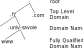
\includegraphics[width=150px]{Images/11_DNSnommage.pdf} \\

Les serveurs DNS ont 2 rôles :
\begin{itemize}
	\item Faire de la résolution
	\item Héberger des informations de zone
\end{itemize}

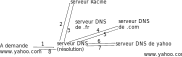
\includegraphics[width=350px]{Images/12_DNSresolution.pdf} \\

Rappel : La durée de mise en cache est renvoyée avec la réponse du serveur DNS hébergeant l'information. \\

\titre{DNS-spoofing} \\
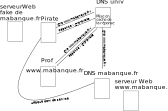
\includegraphics[width=350px]{Images/13_DNSspoofing.pdf} \\
Remarque : les concepteurs de DNS ont prévu cette attaque : une id est ajoutée à la demande afin de s'assurer que celui qui répond est bien celui à qui on a demandé. Problème : ces id sont codés sur 16 bits donc il est devenu facile d'envoyer les 65 535 réponses possibles en un temps très court.\\

\titre{Parade :} On fait intervenir la couche transport pour "compléter" l'id : les 2 protocoles disponibles pour cette couche sont UDP et TCP, ces 2 protocoles ont des champs communs (port source : identifie l'application sur la machine émettrice / port dest : identifie l'application sur la machine réceptrice). Le pirate doit deviner les 16 bits à mettre dans port dest => ça fait 16 + 16 = 32 bits à deviner => 4 milliards de réponses possibles. \\

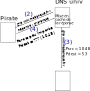
\includegraphics[width=150px]{Images/14_DNSsolution.pdf} 

Remarque : Avant les serveurs DNS mettaient toujours 53 en port dest.

